\section{Explaining Type Errors With Traces}
\label{sec:interactive}

A trace, on its own, is too detailed to be
a good explanation of the type error. One approach
is to use the witness input to step through the
program with a \emph{debugger} to observe how
the program evolves.
%
This route is problematic for two reasons.
%
First, existing debuggers and interpreters for
typed languages (\eg\ \ocaml) typically require
a type-correct program as input.
%
Second, we wish to have a quicker way to get
to the essence of the error, \eg\ by skipping
over irrelevant sub-computations, and focusing
on the important ones.

Next, we present a novel way to debug executions.
%
First, we develop a notion of a \emph{reduction graphs}
and extend our semantics with a form of \emph{tracing}
so that they incrementally collect the edges
in the graph (\S~\ref{sec:inter-semant}).
%
Next, we express a set of common \emph{interactive debugging}
steps as graph traversals (\S~\ref{sec:traversing-graph}), yielding
an novel interactive debugger that allows the user
to effectively visualize \emph{how} the program goes (wrong).

\subsection{Tracing Semantics}
\label{sec:inter-semant}
%
\begin{figure*}[t]
%% \relDescription{Computing Sub-Terms}
%% \begin{gather*}
%% \begin{array}{lcl}
%% \subtermssym                 & \dcolon & e \to \tr \\
%% \subterms{\eapp{e_1}{e_2}}   & \defeq & \subterm{\eapp{e_1}{e_2}}{e_1}; \subterm{\eapp{e_1}{e_2}}{e_2} \\
%% \subterms{\eplus{e_1}{e_2}}   & \defeq & \subterm{\eplus{e_1}{e_2}}{e_1}; \subterm{\eplus{e_1}{e_2}}{e_2} \\
%% \subterms{\eif{e_1}{e_2}{e_3}}   & \defeq & \subterm{\eif{e_1}{e_2}{e_3}}{e_1}; \\
                                %% &        & \subterm{\eif{e_1}{e_2}{e_3}}{e_2}; \\
                                %% &        & \subterm{\eif{e_1}{e_2}{e_3}}{e_3} \\
%% \subterms{\elet{x}{e_1}{e_2}}   & \defeq & \subterm{\elet{x}{e_1}{e_2}}{e_1}; \\
                                %% &        & \subterm{\elet{x}{e_1}{e_2}}{e_2} \\
%% \subterms{\efun{x}{e}}       & \defeq & \subterm{\efun{x}{e}}{e} \\
%% \subterms{e}                 & \defeq & \bullet
%% \end{array}
%% \end{gather*}
\judgementHead{Traced Evaluation}{\stepg{e}{\su}{\tr}{e}{\su}{\tr}}
\begin{gather*}
\inference[\recontext]
  {\stepg{e}{\su}{\tr}{e_1}{\su_1}{\tr_1}}
  {\stepg{C[e]}{\su}{\tr}{C[e_1]}{\su_1}{\singlestep{C[e]}{C[e_1]}; \tr_1}}
\\ \\
\inference[\reappgood]
  {\pair{\efun{x}{e}}{\su_2} = \force{v_1}{\tfun{\thole{}}{\thole{}}}{\su_1}}
  {\stepg{\eapp{v_1}{v_2}}{\su_1}{\tr}
         {e\sub{x}{v_2}}{\su_1;\su_2}{\singlestep{\eapp{v_1}{v_2}}{e\sub{x}{v_2}}; \tr}}
\\ \\
\inference[\reappbad]
  {\pair{\stuck}{\su_2} = \force{v_1}{\tfun{\thole{}}{\thole{}}}{\su_1}}
  {\stepg{\eapp{v_1}{v_2}}{\su_1}{\tr}{\stuck}{\su_1;\su_2}{\singlestep{\eapp{v_1}{v_2}}{\stuck}; \tr}}
\end{gather*}
\caption{A selection of the operational semantics from
  Figure~\ref{fig:operational}, extended to collect a full reduction
  graph.}
\label{fig:interactive}
\end{figure*}

\paragraph{Reduction Graphs}
%
A \emph{steps-to} edge is a pair of expressions \singlestep{e_1}{e_2}, which
intuitively indicates that $e_1$ reduces, in a single step, to $e_2$.
%
%A \emph{sub-term} edge is a pair of expressions \subterm{e_1}{e_2}, which
%intuitively indicates that $e_1$ contains $e_2$ as a sub-expression.
%
A \emph{reduction graph} is a set of steps-to edges:
$$\tr ::= \bullet \spmid \singlestep{e}{e}; \tr$$  %% \spmid \subterm{e}{e}; \tr$$

\paragraph{Tracing Semantics}
%
We extend the transition relation (\S~\ref{sec:semantics}) to
collect the set of edges corresponding to the reduction graph.
%
Concretely, we extend the operational semantics to
a relation of the form $\stepg{e}{\vsu}{\tr}{e'}{\vsu'}{\tr'}$
where $\tr'$ collects the edges of the transition.

\paragraph{Collecting Edges}
%
Next, we describe the general recipe for extending a transition
rule to collect edges.
%
The general recipe for collecting steps-to edges is to
to recording the consequent of each original rule in the
trace. That is, each original judgment \step{e}{\vsu}{e'}{\vsu'}
becomes \stepg{e}{\vsu}{\tr}{e'}{\vsu'}{\singlestep{e}{e'}; \tr}.
%
As the translation is mechanical, we provide a selection of examples
in Figure~\ref{fig:interactive}.

%%% The sub-term edges are delegated to a helper function \subtermssym\
%%% which adds edges from an expression to each of its
%%% \emph{immediate} sub-expressions.
%%% %
%%% We collect \subtermssym\ edges after each transition,
%%% to get the following template for the small-step relation:
%%% \[
%%% \stepg{e}{\vsu}{\tr}{e'}{\vsu'}{\singlestep{e}{e'}; \subterms{e'}; \tr}
%%% \]


\subsection{Interactive Debugging}
\label{sec:traversing-graph}

Next, we show how to build a visual interactive debugger
from the traced semantics, by describing the visualization
\emph{state} \ie\ what the user sees at any given moment,
the set of \emph{commands} available to user and what
they do, and finally how we use a command to \emph{update}
the visualization state. In what follows, for clarity of
exposition, we assume we have a (global) trace:
$\stepg{e_0}{\emptysu}{\bullet}{e_n}{\vsu}{\tr}$, where
$e_0$ and $e_n$ are the \emph{initial} and \emph{final}
expressions respectively.

\paragraph{Visualization State}
%
A \emph{visualization state} $\vstate$ is a \emph{directed graph}
whose vertices are expressions and whose edges are such
that each vertex has at most one predecessor and at most one
successor. In other words, the visualization state looks
like a set of linear lists of expressions as shown in
Figure~\ref{fig:nanomaly-factorial}.
%
The \emph{initial state} is the graph containing a single
edge linking the initial and final expressions.

\paragraph{Visualization Context}
%
The \emph{visualization context} of each expression $e$
in the visualization state $\vstate$ is the (unique) linear chain
in which the expression $e$ belongs.
%
We write $\vroot{\vstate}{e}$ for the \emph{first} (or root)
expression appearing in the visualization context of $e$ in
$\vstate$.

\paragraph{Commands}
Our debugger supports the following \emph{commands}, each of which
is parameterized by a single expression (vertex) selected from the
(current) visualization state:
%
\begin{itemize}
%
\item \stepforwardsym, \stepbackwardsym:
      show the result of a single step forward or backward respectively,
%
\item \jumpforwardsym, \jumpbackwardsym:
      show the result of taking multiple steps (a \emph{``big''} step)
      upto the first beta-reduction forward or backward respectively,
%
\item \stepintosym:
      show the result of stepping into a function call in a sub-term,
      isolating it from the context,

\item \stepoversym:
      show the result of skipping over a function call in a sub-term.
\end{itemize}

\begin{figure*}[t]
\[
\begin{array}{lcl}
\stepforward{\vstate}{e}  & \defeq
  & e' \quad \mbox{where } \singlestep{e}{e'} \in \tr \\ \\

\stepbackward{\vstate}{e} & \defeq
  & e' \quad \mbox{where } \singlestep{e'}{e} \in \tr \mbox{ and } e' \in \vpath{\vstate}{e} \\ \\

\jumpforward{\vstate}{e} & \defeq
  & \begin{cases}
    e'                         & \mbox{if } e' = \eapp{v}{v'} \\
    \jumpforward{\vstate}{e'}  & \text{otherwise}
    \end{cases}
    \mbox{\qquad where } e' = \stepforward{\vstate}{e} \\ \\

\jumpbackward{\vstate}{e} & \defeq
  & \begin{cases}
    e'                         & \mbox{if } e' = \eapp{v}{v'} \\
    \jumpbackward{\vstate}{e'} & \text{otherwise}
    \end{cases}
    \mbox{\qquad where } e' = \stepbackward{\vstate}{e} \\ \\

\stepinto{\vstate}{e} & \defeq
  & e'\sub{x}{v'} \quad \mbox{if } e = C[\eapp{v}{v'}] \mbox{ and } \singlestep{\eapp{v}{v'}}{e'\sub{x}{v'}}  \\ \\

\stepover{\vstate}{e} & \defeq
  & C[v] \quad \mbox{if } e = C[\eapp{v_1}{v_2}] \mbox{ and } \multistep{\eapp{v_1}{v_2}}{v} \in \tr \\[0.25in]

\vpath{\vstate}{e} & \defeq
  & \{e' \spmid \multistep{\vroot{\vstate}{e}}{e'} \in \tr
                \mbox{ and }
                \multistep{e'}{e} \in \tr \} \\[0.15in]
\end{array}
\]
\caption{Rules for computing the \emph{next} term given a
         visualization state $\vstate$, selected term $e$
         and command.}
\label{fig:traversing-graph}
\end{figure*}


\paragraph{Update}
%
Figure~\ref{fig:traversing-graph} shows
how we compute the \emph{next} expression
(to be added to the visualization state)
given the current visualization state
$\vstate$, command $\cmd$ and selected
expression $e$.
%
It is straightforward to then \emph{update}
the visualization graph by adding the new
term before (resp.\ after) the selected
expression $e$ if the command was a step
or jump forward (resp.\ backward), or
to create a new visualization context
if the command was $\stepintosym$.

%%% and \updState{\vstate}{\cmd}{e} then updates the graph
%%% by inserting the new expression appropriately, using
%%% one of the following graph manipulating functions:
%%% %
%%% \putBefore{\vstate}{e}{e'} (resp. \putAfter{\vstate}{e}{e'})
%%% returns the modified version of \vstate\ where $e'$ is the
%%% immediate predecessor of $e$ (resp.\ the immediate successor of $e$);
%%% %
%%% \putRoot{\vstate}{e}{e'} returns the modified version of \vstate
%%% extended with a new root vertex $e$ with successor $e'$.
%%% %
%%% @getNext vs e@ returns the immediate successor of @e@ in $\tr$.
%%% %
%%% @getPrev vs e@ computes the path @p@ between @e@ and its immediate
%%% predecessor in the current visualization, and then returns @e@'s immediate
%%% predecessor along @p@.
%%% %
%%% @getSubterms vs e@ traverses the sub-term edges to decompose an
%%% expression into a list of sub-expressions paired with their context.
%%% %
%%% @applyCtx vs e ctx@ applies @ctx@ to @e@, traversing the sub-term edges
%%% in reverse to find the super-term of @e@.
%%% %
%%% \hbox{@findApp vs e@} builds on top of @getSubterms@ to find the first
%%% application sub-term (if any), \ie the first sub-term that looks like
%%% $\eapp{v_1}{v_2}$.
%%% %
%%% @findVal vs e@ traverses the single-step edges to find the final value
%%% that @e@ reduces to.

\begin{figure}[t]
\centering
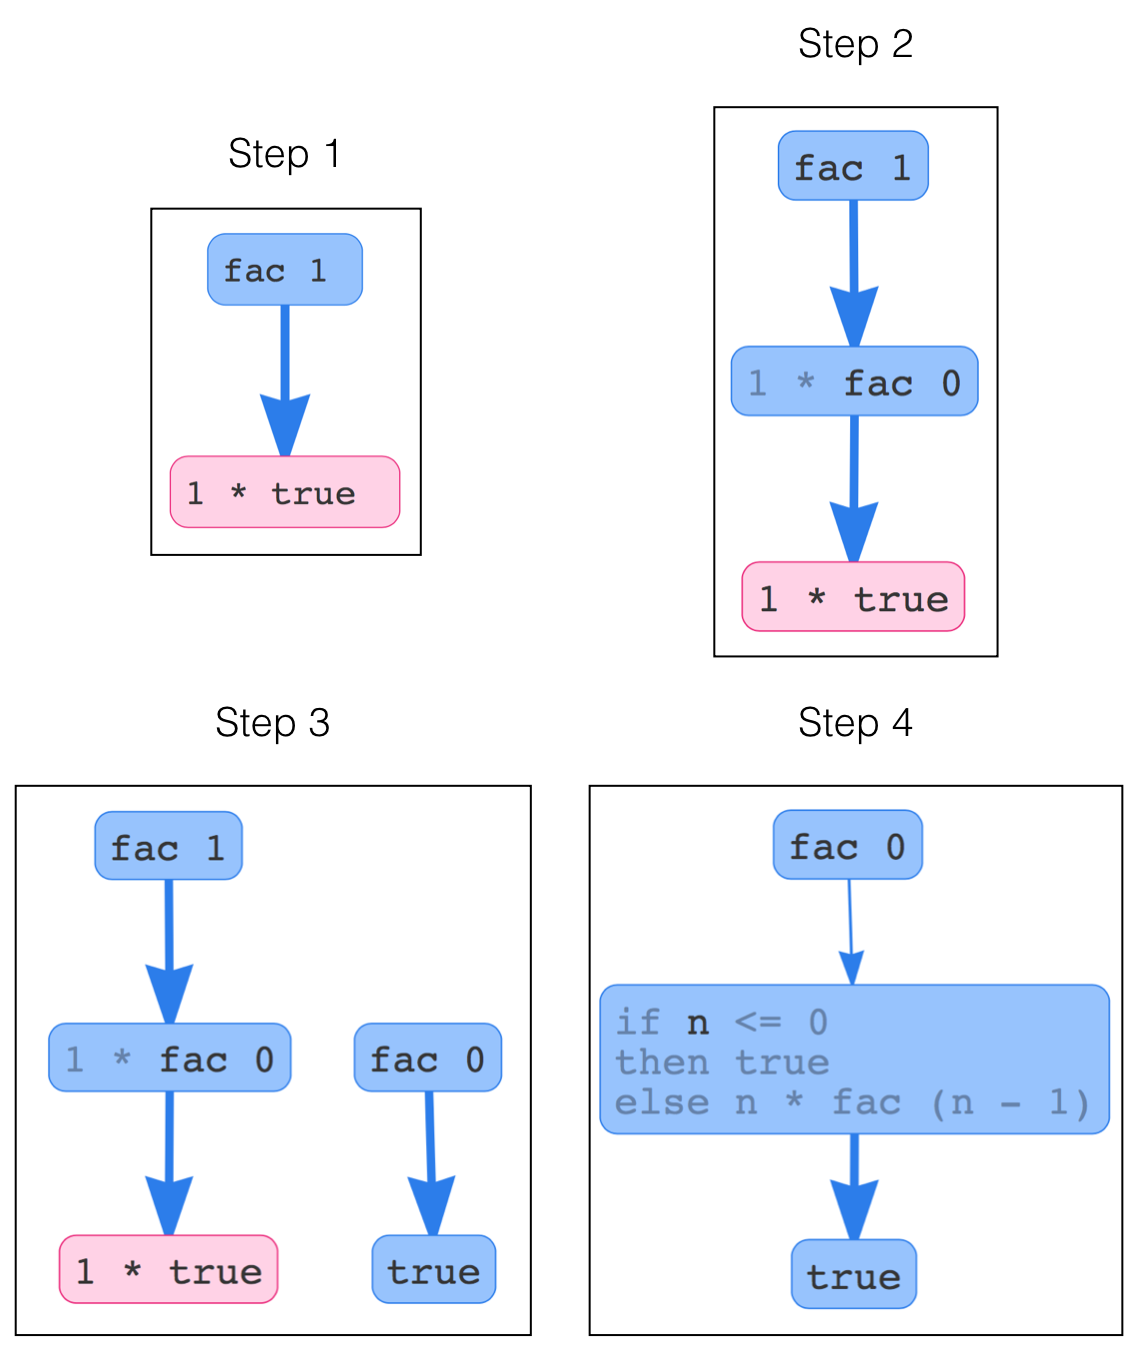
\includegraphics[width=\linewidth]{fac-steps-new.png}
\caption{A sequence of interactions with the trace of
  \texttt{fac 1}. The stuck term is red, in each node the redex is
  highlighted. Thick arrows denote a multi-step transition, thin arrows
  denote a single-step transition. We start in step 1. In step 2 we jump
  forward from the witness to the next function call. In step 3 we step
  into the recursive \texttt{fac 0} call, which spawns a new ``thread''
  of execution. In step 4 we take a single step forward from
  \texttt{fac 0}.}
\label{fig:nanomaly-factorial}
\end{figure}
